\documentclass[a4paper]{article}

%% Language and font encodings
\usepackage[english]{babel}
\usepackage[utf8x]{inputenc}

\usepackage{booktabs}
\usepackage{tabu}
\usepackage[T1]{fontenc}

%% Sets page size and margins
\usepackage[a4paper,top=3cm,bottom=2cm,left=3cm,right=3cm,marginparwidth=1.75cm]{geometry}

%% Useful packages
\usepackage{amsmath}
\usepackage{graphicx}
\usepackage{titling}
%\usepackage{apacite}
\usepackage[colorinlistoftodos]{todonotes}
\usepackage[colorlinks=true, allcolors=blue]{hyperref}
\usepackage[strings]{underscore}


\title{Modeling and 3D Printing Sea Shells\\
		\large Final Report}
\author{Edward Ye || 100972832}
\date{2019/04/22}

\begin{document}
\maketitle

\begin{abstract}
	I thought sea shells were cool so I made some models and 3D printed them.
\end{abstract}

\tableofcontents

\section{Some Background and Motivation}

Sea shells have interesting patterns which  appear to be readily described by mathematics and computation. Work has already been done to describe aspects of sea shells, from the spiral shape to the color patterns to the protrusions found on the exterior \cite{Galbraith00modelingmurex}\cite{abss}\cite{VANDERHELM1998505}. Recently some work has also gone into the 3D printing of sea shell model \cite{3dprinting-seashells}\cite{bachman-3dprinting}.

The motivation of this project will be to extend the methods of generating the exterior protrusions to be able to mimic a wider variety of shells. Prusinkiewicz and Fowler have modeled periodic ridge and bump patterns and they have also combined multiple generating curves to imitate more intricate shells \cite{abss}. Galbraith et al. have used constructive solid geometry (CSG) to compose different modules to generate a complete Murex Cabritii model. They have proposed the use of reaction-diffusion (RD) to place protrusions algorithmically \cite{Galbraith00modelingmurex}. Intuitively this appears to be a reasonable idea since the protrusion placement of certain shells are something like the placement of spots upon a leopard. Such patterns have already been described as textures using RD \cite{Turk:1991:GTA:127719.122749}.

\subsection{Main Objective}

An interesting candidate for such a method would be:

\begin{figure}[h]
	\centering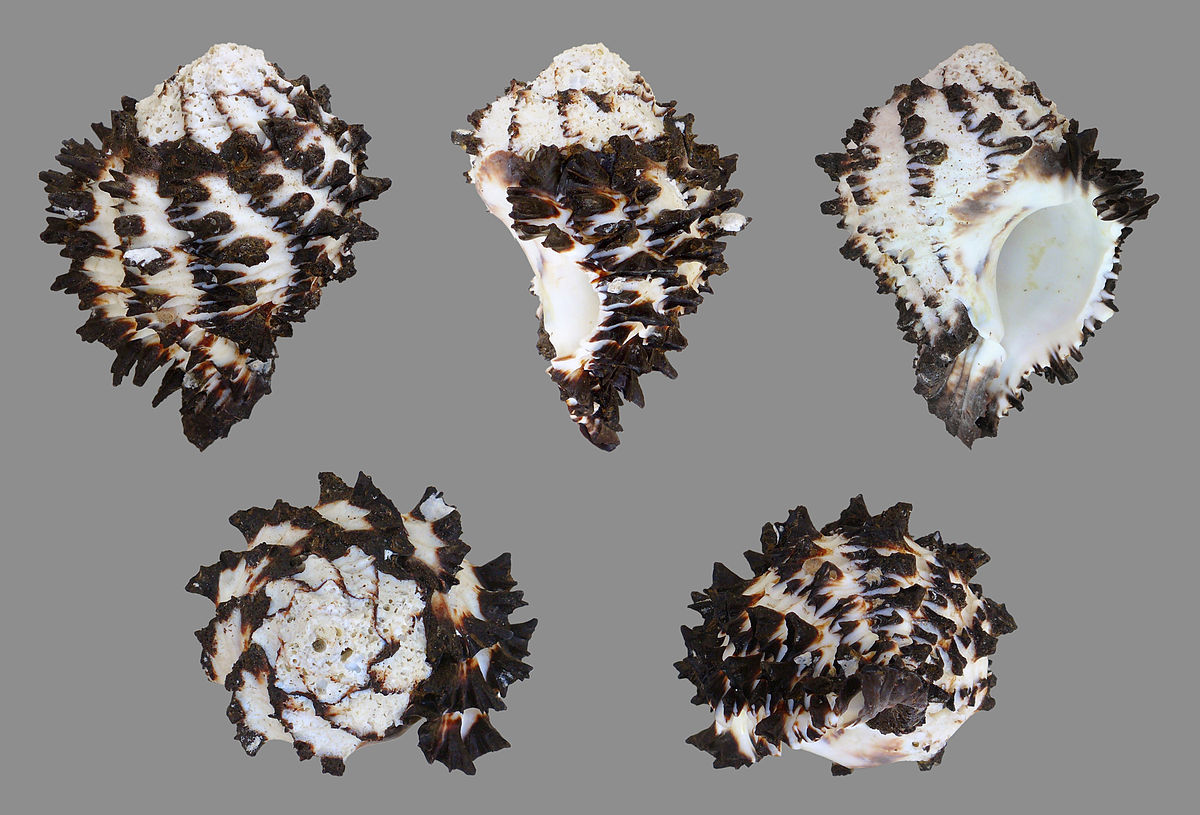
\includegraphics[scale=0.25]{./img/hexaplex_radix.jpg}
	\caption{Hexaplex radix \cite{wikipedia-hexaplex}}
	\label{fig:hexaplex-radix} % Unique label used for referencing the figure in-text
	%\addcontentsline{toc}{figure}{Figure \ref{fig:placeholder}} % Uncomment to add the figure to the table of contents
\end{figure}

The main objective would be to create a model that closely resembles the shell and to 3D print it. After completing the main objective it may be possible to generalize the methods used to describe various other shells.

\section{Implicit Surface}

The initial idea was to use a raytracer, such as POV-Ray, to create an implicit surface (isosurface in POV-Ray terminology) that would represent the shell model. The software allows for textures to also act as functions, so that the sum of the implicit equation and the texture function would generate the desired surface. POV-Ray could then generate a point cloud that would form a mesh to be 3-D printed.

\subsection{Logarithmic Spiral}

Shells are modeled by logarithmic spirals. In polar coordinates the logarithmic spiral equation is:

\begin{equation}
	r = Ae^{\alpha \theta}
\end{equation}

Where $A$ shifts the position of the spiral inward or outward, and $\alpha$ multiples the growth rate $(\frac{dr}{d\theta} = \alpha A e^{\alpha \theta} = \alpha r)$.

\begin{figure}[h]
	\centering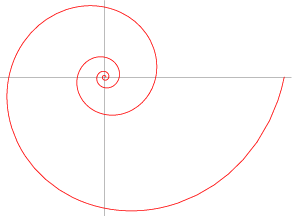
\includegraphics[scale=0.7]{./img/logarithmic-spiral.png}
	\caption{2-D Logarithmic Spiral using equation (1). \cite{logspiral}}
	\label{fig:log-spiral} % Unique label used for referencing the figure in-text
	%\addcontentsline{toc}{figure}{Figure \ref{fig:placeholder}} % Uncomment to add the figure to the table of contents
\end{figure}

\pagebreak

In 3-D Cartesian coordinates (1) can be represented as:

$$ r = \sqrt{x^2 + y^2 + z^2 } $$
$$ \theta = tan^{-1}({\frac{y}{x}}) $$

\begin{equation}
	\sqrt{x^2 + y^2 + z^2 } = A e^{\alpha \cdot tan^{-1}({\frac{y}{x}})}
\end{equation}

Squaring both sides of (2) then gives the implicit equation:

\begin{equation}
	s(x,y,z) = x^2 + y^2 + z^2 - A e^{2 \alpha \cdot tan^{-1}({\frac{y}{x}})} = 0
\end{equation}

\begin{figure}[h]
	\centering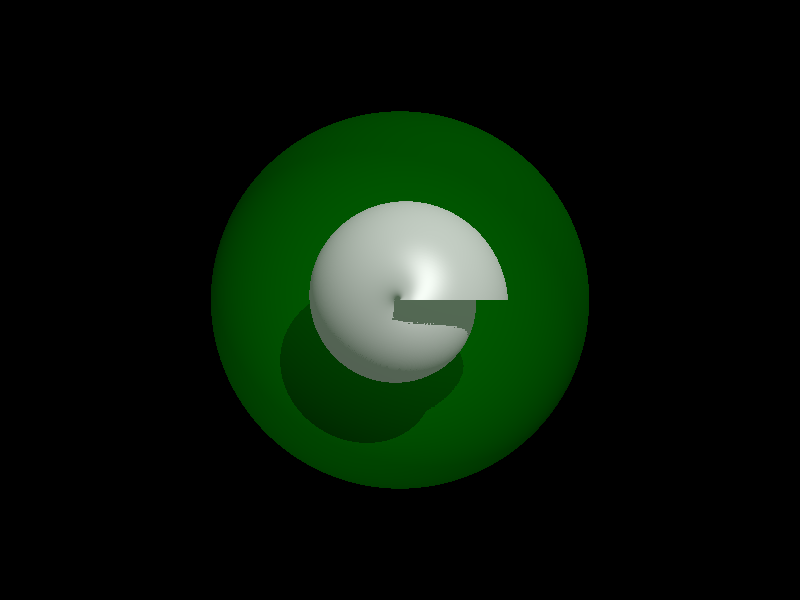
\includegraphics[scale=0.3]{./img/logspiral.png}
	\caption{3-D log spiral generated by \textit{logspiral.pov} using an implementation of equation (3).}
	\label{fig:3d-log-spiral} % Unique label used for referencing the figure in-text
	%\addcontentsline{toc}{figure}{Figure \ref{fig:placeholder}} % Uncomment to add the figure to the table of contents
\end{figure}

If I have some other function, such as $f_{noise}(x,y,z)$, I can add it to equation (3) to get another implicit equation:

\begin{equation}
	s(x,y,z) + f_{noise}(x,y,z) = 0
\end{equation}

\begin{figure}[h]
	\centering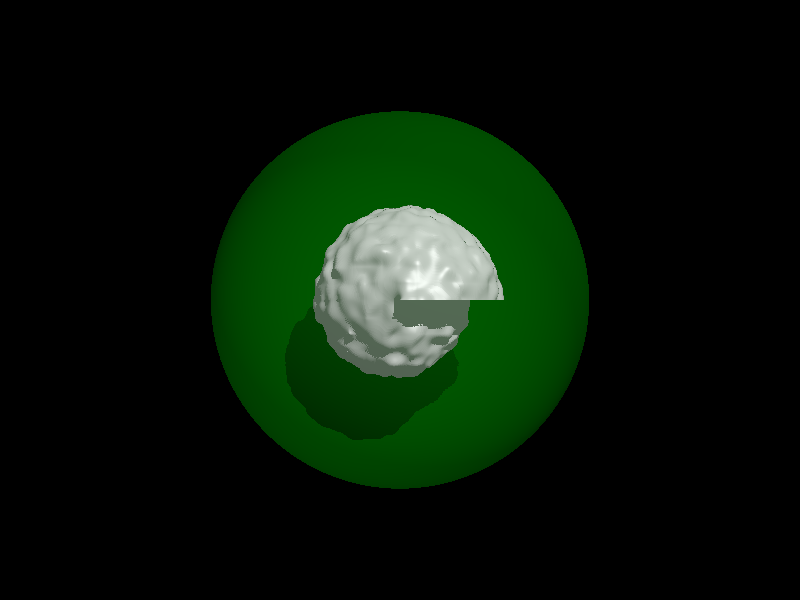
\includegraphics[scale=0.3]{./img/logspiral_noise.png}
	\caption{Equation (4) gives something pretty ugly.}
	\label{fig:3d-log-spiral-noise} % Unique label used for referencing the figure in-text
	%\addcontentsline{toc}{figure}{Figure \ref{fig:placeholder}} % Uncomment to add the figure to the table of contents
\end{figure}

After fiddling around with this for a while it became apparent that the existing parametric equations describing shells could not be easily turned into implicit equations.

\section{Parametric Equations}

In \cite{JORGEPICADO} a 14 parameter parametric equation is used to model sea shells.

\subsection{14 Parameters} 

\subsection{Processing}

\subsection{Blender}

\section{Reaction Diffusion Shaders}

\section{Conclusion}

\subsection{Future Work}

\bibliographystyle{plain}
\bibliography{refs}

\end{document}